 %%%%%%%%%%%%%%%%%%%%%%% file template.tex %%%%%%%%%%%%%%%%%%%%%%%%%
%
% This is a general template file for the LaTeX package SVJour3
% for Springer journals.          Springer Heidelberg 2010/09/16
%
% Copy it to a new file with a new name and use it as the basis
% for your article. Delete % signs as needed.
%
% This template includes a few options for different layouts and
% content for various journals. Please consult a previous issue of
% your journal as needed.
%
%%%%%%%%%%%%%%%%%%%%%%%%%%%%%%%%%%%%%%%%%%%%%%%%%%%%%%%%%%%%%%%%%%%
%
% First comes an example EPS file -- just ignore it and
% proceed on the \documentclass line
% your LaTeX will extract the file if required
\begin{filecontents*}{example.eps}
%!PS-Adobe-3.0 EPSF-3.0
%%BoundingBox: 19 19 221 221
%%CreationDate: Mon Sep 29 1997
%%Creator: programmed by hand (JK)
%%EndComments
gsave
newpath
  20 20 moveto
  20 220 lineto
  220 220 lineto
  220 20 lineto
closepath
2 setlinewidth
gsave
  .4 setgray fill
grestore
stroke
grestore
\end{filecontents*}
%
\RequirePackage{fix-cm}

%
%\documentclass{svjour3}                     % onecolumn (standard format)
%\documentclass[smallcondensed]{svjour3}     % onecolumn (ditto)
%\documentclass[smallextended]{svjour3}       % onecolumn (second format)
\documentclass[twocolumn]{svjour3}          % twocolumn
%
\smartqed  % flush right qed marks, e.g. at end of proof
%
\usepackage{graphicx}
\usepackage{subfigure}
\usepackage{booktabs} % For formal tables
\usepackage[ruled]{algorithm2e} % For algorithms
\usepackage{multirow}
\newcommand{\tabincell}[2]{\begin{tabular}{@{}#1@{}}#2\end{tabular}}
%
% \usepackage{mathptmx}      % use Times fonts if available on your TeX system
%
% insert here the call for the packages your document requires
%\usepackage{latexsym}
% etc.
%
% please place your own definitions here and don't use \def but
% \newcommand{}{}
%
% Insert the name of "your journal" with
% \journalname{myjournal}
%
\begin{document}

\title{DAL-SMC: Distributed Statistical Model Checking with Abstraction and Learning
\thanks{This work was supported by NSFC (Grant No.61472140, 61202104).}
}
%\subtitle{Do you have a subtitle?\\ If so, write it here}

%\titlerunning{Short form of title}        % if too long for running head

\author{Kaiqiang Jiang \and Yi Ao \and Ping Huang \and Hui Zan \and Dehui Du}

%\authorrunning{Short form of author list} % if too long for running head

\institute{East China Normal University, Shanghai Key Laboratory of Trustworthy Computing \\
              School of Computer Science and Software Engineering, Shanghai, China\\
              %Tel.: +123-45-678910\\
              %Fax: +123-45-678910\\
              \email{dhdu@sei.ecnu.edu.cn}           %  \\
%             \emph{Present address:} of F. Author  %  if needed
}

\date{Received: date / Accepted: date}
% The correct dates will be entered by the editor


\maketitle

\begin{abstract}
The core idea of Statistical Model Checking (SMC) is to decide whether the stochastic model satisfies a given property or to evaluate its probability of satisfaction by combining statistical techniques with Monte-Carlo simulation on model traces. However, SMC still encounters performance bottleneck due to the consumption of the extremely large number of traces, each of which itself could be extremely time-consuming. To solve these problems, we have proposed an optimized SMC approach called AL-SMC to reduce the number of traces in our previous work. In order to reduce the time consumption for generating a single trace further, we propose a general framework for distributed SMC based on master/slaves architecture without introducing bias. A series of algorithms are introduced to show that bayesian interval estimation (BIE) algorithm and AL-SMC are easily parallelizable on our general framework. Besides, we propose parameter optimization approach with a genetic algorithm to reduce the statistical error of distributed AL-SMC (DAL-SMC). We also implemented DAL-SMC algorithms in our ModanaOnline platform to support the automatic process. To illustrate the feasibility of our approach, three benchmarks are presented to compare the number of simulation traces, time consumption and statistical error between DAL-SMC and classic SMC algorithms. The experiment results show that the time consumption of our toolset is effectively reduced and the accuracy is ensured within an acceptable error bound.
\keywords{Statistical model checking \and Statistical abstraction \and Learning \and Distributed technology \and Bayesian interval estimation algorithm}
% \PACS{PACS code1 \and PACS code2 \and more}
% \subclass{MSC code1 \and MSC code2 \and more}
\end{abstract}


\section{Introduction}

\textit{Cyber-physical systems} (CPS) are integration of computation with physical processes whose behavior is defined by both computational and physical parts of the system \cite{Zanero17}. Embedded computers and networks monitor and control the physical processes, usually with feedback loops where physical processes affect computations and vice versa. The heterogeneity is one of the main characteristics of CPS. The components of CPS are of various types, requiring interfacing and interoperability across multiple platforms and different models of computation. Verifying coordination of heterogeneous CPS is a challenging problem. The coordination between heterogeneous components of CPS could be implemented with Functional Mock-up Interface (FMI) based co-simulation technology. The FMI standard was first developed in the MODELISAR project started in 2008 and supported by a large number of software companies and research centers \cite{ClauMODELISAR}. FMI supports simulation of complex systems composed of heterogeneous components, by coupling different models with their own solvers in a co-simulation environment.

In this paper, we focus on verifying the coordination of CPS which implemented with FMI 2.0 \cite{Cremona2006Automatic} based co-simulation. The key point is Master Algorithm (MA) \cite{AckerDVM15} and connector configuration between Functional Mock-up Units (FMUs) \cite{Tripakis15}, which specifies the orchestration and the exchange of data among FMUs during the whole coordination process. To ensure the correctness of coordination, we need to verify MA and connector configuration with model checking. However, MA is not a part of FMI standard. This implies that the user or tool vendor needs to develop a sophisticated orchestration algorithm for the problem at hand. 
%Is the MA deadlock free?
%Dose the MA satisfy the reachability? To solve these problem, we can verify the MAs with model checking technology.
There are three versions of MA \cite{BromanBGLMTW13}: fixed step algorithm, rollback algorithm and predictable step size algorithm. Rollback and predictable step size algorithms are based on the extension of FMI 2.0, which supports the rollback and a predict function. P.G. Larsen et al. \cite{Larsen2016Integrated} formally analysed the fixed step and rollback algorithms with the FDR3 refinement checker. However, there still lacks effective approach to verify the whole FMI-based coordination process. Based on our previous work \cite{LiuJWCD16}, we found that the simulation process of coordination is time-intensive. Therefore, it is reasonable to formalize the coordination with Timed Automaton (TA) \cite{BehrmannDLHPYH06}, which is the classic formalism for modeling real-time system. 
In this paper, we propose to model the MA with TA and verify the correctness of MA. Furthermore, we also attempt to encode the components of CPS with TA and verify the architecture of whole system with the model checker UPPAAL \cite{BehrmannDLHPYH06}. 
%To achieve our goal, we propose a novel approach to model check the coordination of CPS with TA.

\textbf{In summary, our main contributions are as follows}:
\begin{itemize}
\item
We propose a novel approach to verify the coordination of CPS with model checking. To bridge the gap between FMU and the model checker, we propose some encoding rules to encode FMU as TA.
\item
We model and verify three various MAs to ensure the correctness of the coordination. With the help of UPPAAL, we analyse the reachability, livelock and deadlock of three versions of MA.
%\item
%We present a novel approach to model check several properties of the co-simulation based on timed automata. With the help of model checker, the property such as livelock, deadlock and reachability of the co-simulation are verified. 
\item
The prototype for model checking coordination of CPS is under developing, which is integrated in our Modana platform \cite{Cheng2015Modana}. We have implemented the \textit{SysML modeling environment} and the \textit{co-simulator} to simulate CPS in Modana (https://github.com/ECNU-MODANA/AL-Modana.git) \cite{Fritzson1998Modelica}.
\end{itemize}
The main novelty of our work, compared with the previous work, is that we propose to verify coordination of CPS with TA-based model checking. As far as we know, there is few existing approaches supporting TA-based model checking for the coordination of CPS.

The remainder of this paper is organized as follows. In Section~\ref{sec:fmi}, we briefly review the technical background including FMI, FMU and TA. Then, we present the technical road map of our approach and discuss how to encode FMU as TA with the help of their semantic mapping rules in Section~\ref{sec:encoding}. In Section~\ref{sec:ma}, we model three versions of MA with TA and verify their properties such as the livelock and deadlock. Section~\ref{sec:sysml} presents a case study to demonstrate the feasibility of our approach. We model the architecture of water tank system with SysML Block Definition Diagram (BDD) \cite{SemerathBHSV17}, and then obtain the FMU component of each block and the connection between FMUs. We encode the FMUs of water tank with TA and verify the correctness of the coordination between components of water tank system with UPPAAL. Finally, we position our work with respect to related work before concluding and discussing possible future extensions.




















%The syntax of TA is as follows:
%\par
%\textbf{Timed Automata}
%A timed automata over a finite set of clocks $C$ and a finite set of actions $Sigma$ is a quintuple $\textit{H}=(L,l_{0},\Sigma,E,I)$, where
%\begin{itemize}
%\item
%$L$ is a finite set of locations,
%\item
%$l_{0}\in L$ is the initial location,
%\item
%$\Sigma$ is a finite set of actions, and $\Sigma=\Sigma_{i}+\Sigma_{o}$, where $\Sigma_{i}$ is the set of input actions, $\Sigma_{o}$ is the set of output actions,
%\item
%$E$ is a finite set of transactions, where $E\subseteq L \times \mathcal{B(C)}\times \Sigma \times 2^C\times L$
%\item
%$I:L\rightarrow \mathcal{B(C)})$ assigns invariants to locations.
%\end{itemize}
\section{Distributed bayesian interval estimation and DAL-SMC}

In this section, we first introduce the general framework of distributed SMC based on master/slaves architecture. Next, we apply the framework to BIE algorithm and present the core algorithms of distributed BIE. With the help of distributed BIE, the time for generating a single trace is reduced. Besides, in order to reduce the number of traces generated by distributed BIE, we propose the DAL-SMC technique and present the core algorithms of DAL-SMC, which is an improvement of distributed BIE. However, we found that DAL-SMC has large statistical error compared with distributed BIE. To solve this problem, we propose the parameter optimization with genetic algorithm to reduce the statistical error of DAL-SMC.

\subsection{Framework of distributed SMC}

SMC encounters the performance bottleneck in that the high confidence required by an answer may demand large number of traces, each of which itself may be time-consuming. Fortunately, we find that statistical methods which use independent traces are trivially parallelizable. Therefore, we can solve this problem by parallel computation based on master/slaves architecture (Figure \ref{fra}): multiple slave processes register their abilities to generate traces. The master process is used to collect traces and perform the statistical test. When using distributed sampling with sequential test, the number of simulation traces is unknown in advance. Therefore, it is important to avoid introducing bias when collecting the traces generated by the slave processes. To solve this problem, we adopt the method proposed in \cite{Bulychev2012Checking} which aggregates traces by batches and a buffer.

\begin{figure}[htbp]
\centering{
		\subfigure[Distributed architecture for trace generations]{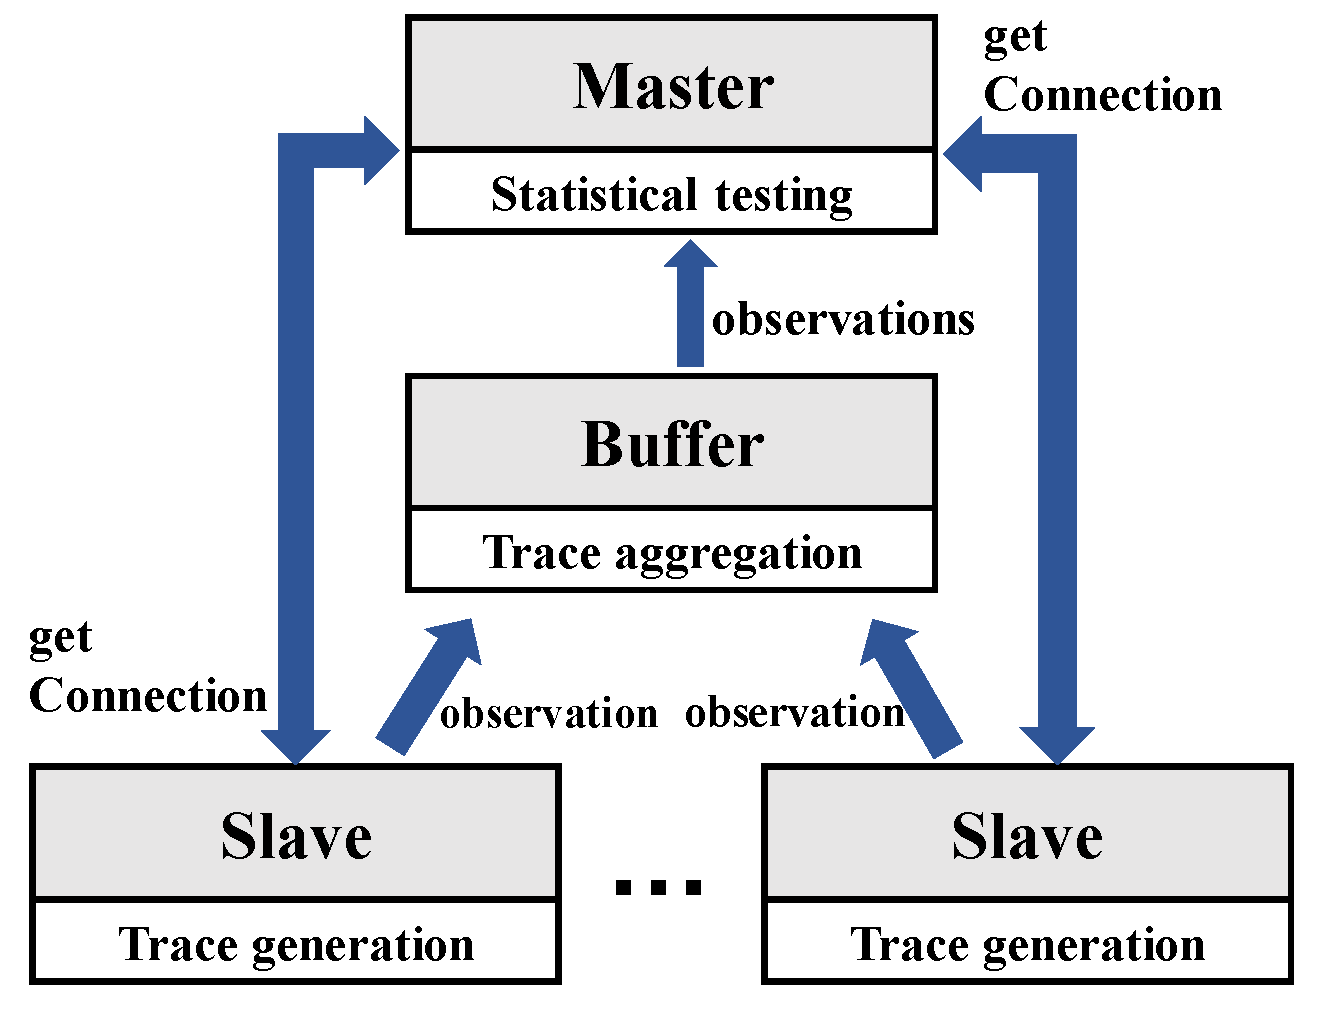
\includegraphics[width=2.5in,height=2.0in]{fig/slave-master-ach.png}
			\label{fra}}
		\hfil
		\subfigure[Communication protocol]{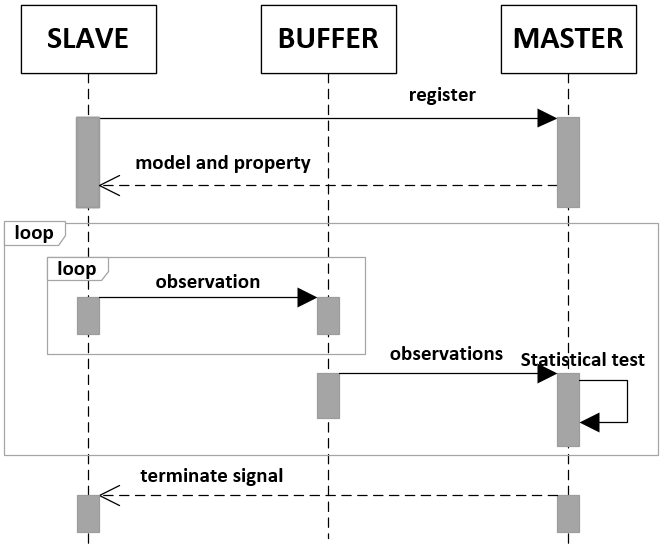
\includegraphics[width=2.5in,height=2.0in]{fig/slave-master-seq.png}
			\label{dsmc}}
	\caption{Framework of distributed SMC.}
	\label{fra_dsmc}
	}
\end{figure}

For Unified Temporal Stochastic Logic (UTSL) model checking \cite{Younes2004Planning}, each observation involves the generation of a trajectory prefix through the discrete event simulation and the verification of a path formula over the generated trajectory prefix. Figure \ref{dsmc} illustrates the communication protocol of distributed acceptance sampling: (i)Multiple slave processes register their abilities with the master process. The master process sends the model and property to the slaves. (ii)The slave processes generate observations and send them to the buffer which is used to aggregate observations, and then the buffer send observations to the master. (iii)The master process executes statistical test. Until the statistical test terminates, it sends terminate signal to the slaves. The framework of distributed SMC is general and flexible. Based on the framework, we present our distributed BIE algorithm in the next subsection. Actually, you can adopt the framework to any other SMC algorithm, not just limits to BIE.

\subsection{Distributed bayesian interval estimation}

We can compute an interval estimate of $p=Prob(M\models\phi)$ with BIE which is a faster statistical model checking algorithm based on estimation. $\phi$ is a Probabilistic Bounded Linear Temporal Logic (PBLTL) formula \cite{baier2008principles}. $M$ is a Stochastic Hybrid Automata (SHA) model \cite{David2014Statistical}. BIE algorithm (Algorithm \ref{alg:bie}) iteratively generates trace, verifies whether it satisfies $\phi$, and then calls statistical test algorithm (Algorithm \ref{alg:sta}) to compute the estimate probability $p'$, interval ($t_0$, $t_1$) of width 2$\delta$ and posterior probability $\gamma$. Until $\gamma >= c$, the algorithm terminates and returns $t_0$, $t_1$ and $p'$, otherwise it generates another trace and repeats.

% Algorithm
\begin{algorithm}[t]
%\SetAlgoNoLine
\KwIn{BLTL property $\phi$, half-interval size $\delta \in (0, 1/2)$, interval coverage coefficient $c \in (1/2, 1)$, Prior Beta distribution with parameters $\alpha$,$\beta$ for the (unknown) probability $p$ that the system satisfies $\phi$}
\KwOut{An interval ($t_0$, $t_1$) of width 2 $\delta$ with posterior probability at least $c$, estimate $p'$ for the true probability $p$}
$x$ = 0; $n$ = 0\;
\Repeat{$\gamma >= c$}{
        $\sigma$ = draw a simulation of the model\;
        \If{$\sigma\models\phi$\; }
        {
           $x$ = $x$ + 1\;
         }
        $n$ = $n$ + 1\;
        $t_0$,$t_1$,$p'$,$\gamma$ = \textbf{CallAlgorithm\ref{alg:sta}($\delta$, $\alpha$,$\beta$,$x$, $n$)};
      }
\caption{Bayesian estimation algorithm}
\label{alg:bie}
\end{algorithm}


% Algorithm
\begin{algorithm}[t]
%\SetAlgoNoLine
\KwIn{half-interval size $\delta$, $\alpha$, $\beta$, positive trace number $x$, total trace number $n$}
\KwOut{An interval ($t_0$, $t_1$) of width 2$\delta$, estimate probability $p'$, posterior probability $\gamma$}
        $p'$ = (x+$\alpha$)/(n+$\alpha$+$\beta$)\;
        ($t_0$, $t_1$) = ($p^,$-$\delta$,$p^,$+$\delta$)\;
        \eIf{$t_1 > 1$ \;}
        {
           ($t_0$, $t_1$) = (1-2$\delta$,1)\;
         }{
        \If{$t_0 > 0$ \;}{
            ($t_0$, $t_1$) = (0,2$\delta$)\;
        }
          }
        $\gamma=\int_{t_0}^{t_1} {f(u|x_1,...,x_n)du}$\;
\caption{Statistical test algorithm}
\label{alg:sta}
\end{algorithm}

Based on the BIE algorithm, we implement distributed BIE algorithm with the help of our distributed SMC framework. Algorithm \ref{alg:dbeas} is the slave algorithm of distributed BIE. $B$ is the size of batch which aggregates the outcomes $x$ to reduce communication. The algorithm iteratively generates trace and verifies whether it satisfies $\phi$. Until $runs == B$, the algorithm terminates and returns the number of positive traces $sats$, otherwise it generates another trace and repeats.

% Algorithm
\begin{algorithm}[t]
%\SetAlgoNoLine
\KwIn{BLTL property $\phi$, model $M$, batch size $B$}
\KwOut{The number of positive traces $sats$}
$sats$ = 0, $runs$ = 0\;
\Repeat{$runs$ == B}{
        $\sigma$ := getSimulationTrace($M$)\;
        \If{$\sigma \models \phi$\; }
        {
           $sats$ ++\;
         }
        $runs$ ++ \;
      }
\caption{Slave algorithm of distributed BIE}
\label{alg:dbeas}
\end{algorithm}

Algorithm \ref{alg:dbeam} is the master algorithm of distributed BIE. \emph{$K$} is the size of buffer which is used to improve concurrency since the slaves can do \emph{$K$} runs ahead of the slowest slave, and \emph{$N$} is the number of slaves. The main steps of master algorithm are as follows: (i)The slave processes register their abilities with the master. The master sends model and property to the slaves. (ii)The master algorithm chooses a slave process randomly, and then it updates batch and buffer only if the buffer size of the slave is smaller than \emph{$K$}. (iii)If the buffers of all slaves are not empty, the algorithm updates the value of \emph{$n$} and \emph{$x$}. (iv)Call algorithm \ref{alg:sta} to compute the estimate probability $p'$, interval ($t_0$, $t_1$) of width 2$\delta$ and posterior probability $\gamma$. Until $\gamma >= c$, the algorithm terminates and returns $t_0$, $t_1$ and $p'$, otherwise it repeats step (ii), (iii) and (iv).

\begin{algorithm}[t]
%\SetAlgoNoLine
\KwIn{BLTL property $\phi$, model $M$, half-interval size $\delta \in (0, 1/2)$, interval coverage coefficient $c \in (1/2, 1)$, Prior Beta distribution with parameters $\alpha$,$\beta$ for the (unknown) probability $p$ that the system satisfies $\phi$, buffer size $K$, batch size $B$, the number of nodes $N$}
\KwOut{An interval ($t_0$, $t_1$) of width 2 $\delta$ with posterior probability at least $c$, estimate $p'$ for the true probability $p$}
$x$ = 0; $n$ = 0\;
batch[0...N-1][0...K-1], buffer[0...K-1], slave[0...N-1]\;
\For{slave[i] $\in$ slave[0...N]}{
getConnection(slave[i])\;
sendModelandProperty($M$,$\phi$,slave[i])\;
}
\Repeat{$\gamma >= c$}{
        node = random(0,$N$-1)\;
        \If{$buffer[node] < K$\; }
        {
           batch[node][buffer[node]] = \textbf{CallAlgorithm\ref{alg:dbeas}(node)}\;
           buffer[node]++\;
         }
        \If{$forall(i < N) buffer[i] > 0$ \; }{
         \For{$i < N$}{
              x += batch[i][0]\;
              n += B\;
             buffer[i]--\;
              batch[i][buffer[i]] = 0\;
            }
         }
         $t_0$,$t_1$,$p'$,$\gamma$ = \textbf{CallAlgorithm\ref{alg:sta}($\delta$, $\alpha$,$\beta$ $x$, $n$)};\;
      }
\caption{Master algorithm of distributed BIE}
\label{alg:dbeam}
\end{algorithm}


\subsection{Distributed AL-SMC}
BIE algorithm has its shortcoming, because it needs more traces when it verifies the property whose probability is close to 0.5 \cite{zuliani2013bayesian}. We have proposed AL-SMC technique to solve this problem in our recent work \cite{jiangkaiqiang2016}. The framework of AL-SMC is shown in Figure \ref{al-smc}. AL-SMC includes three main steps: (i)Sample traces are drawn from the model and input into the abstraction process to obtain abstract traces. The abstraction process includes three steps: \textbf{property-based projection, PCA-based dimension reduction \cite{dunteman1989principal} and key states extraction}. (ii)\textbf{Building and optimization of Prefix Frequency Tree (PFT)} applies the learning technique \cite{carrasco1994learning} to construct optimized PFT with abstract traces. By means of PFT, the original probability space is divided into several \textbf{sub-spaces}. (iii)\textbf{Proba
bility evaluation via multi-BIE} invokes multiple BIE algorithms to evaluate the probabilities of sub-spaces in parallel. The detail of AL-SMC can be found in \cite{jiangkaiqiang2016}.

\begin{figure}[htbp]
	\centering	{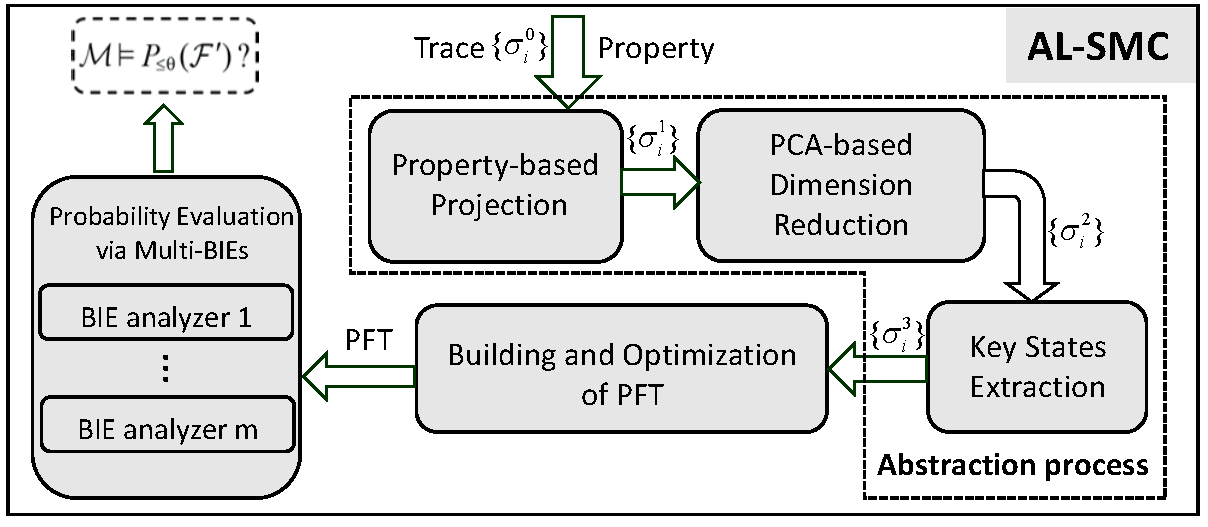
\includegraphics[width=3.2in,height=1.5in]{fig/ALSMC.png}}
	%\vspace{0.10in}
	\caption{The framework of AL-SMC.}\label{al-smc}
\end{figure}

AL-SMC reduces the number of simulation traces compared with BIE algorithm, especially the verification result is close to 0.5. Therefore, the number of traces and the time consumption for generating a single trace will be effectively reduced if we apply the distributed SMC framework into AL-SMC. Fortunately, we find that AL-SMC can be  parallelized with our distributed SMC framework. Therefore, we propose DAL-SMC, whose core algorithms are shown in Algorithm \ref{alg:dalm} and Algorithm \ref{alg:dals}.

Algorithm \ref{alg:dalm} is the master algorithm of DAL-SMC, where $SN$ is the number of sample traces in abstraction process. The master algorithm contains the following steps: (i)The master process generates a set of sample traces $\sigma[0...SN-1]$ which are fed to abstraction process to obtain a set of abstract traces $\sigma'[0...SN-1]$. And then, the optimized PFT is constructed with $\sigma'[0...SN-1]$. (ii)The slave processes get connection with the master. The master process sends model, property and PFT to the slaves. (iii)The algorithm chooses a slave randomly, and then updates $batch[i][j]$ only if the buffer size of this slave is smaller than $K$. (iv)If the buffers of all slaves are not empty, the algorithm evaluates the probability and obtains $p'[j]$ and $\gamma[j]$ of each sub-space. If $\gamma[j] > c$, the evaluation of jth sub-space is terminated. (v)Until the evaluation of all sub-spaces are terminated, the algorithm estimates the probability of the whole space with $p' := \sum\limits_{i=0}^{S-1} p[i]$, otherwise it repeats step (iii), (iv) and (v).

\begin{algorithm}[t]
%\SetAlgoNoLine
\KwIn{BLTL property $\phi$, model $M$, half-interval size $\delta \in (0, 1/2)$, interval coverage coefficient $c \in (1/2, 1)$, Prior Beta distribution with parameters $\alpha$, $\beta$ for the (unknown) probability $p$ that the system satisfies $\phi$, buffer size $K$, batch size $B$, the number of nodes $N$, the number of sample traces $SN$ }
\KwOut{Prefix frequency tree $T$, estimate $p'$ for the true probability $p$}
$\sigma[0...SN-1]$ = getSampleTraces($M$)\;
$\sigma'[0...SN-1]$ = abstractTraces($\sigma[0...SN-1]$)\;
$T$ = ConstructPFT($\sigma'[0...SN-1]$)\;
$d$ = getSubSpacesNum($T$)\;
\For{slave[i] $\in$ slave[0...N]}{
getConnection(slave[i])\;
sendModelandPropertyandPFT($M$,$\phi$,$T$,slave[i])\;
}
x[0...d-1], n\;
batch[0...N-1][0...K-1][0...d-1], buffer[0...K-1], slave[0...N-1]\;
\Repeat{forall(ter[i] $\in$ ter[0...d-1])==true}{
        node = random(0,$N$-1)\;
        \If{$buffer[node] < K$ \; }
        {
           batch[node][buffer[node]][0...d-1] = \textbf{CallAlgorithm\ref{alg:dals}(node)}\;
           buffer[node]++\;
         }
        \If{$forall(i < N) buffer[i] > 0$ \; }{
         \For{$i < N$}{
              x[0...d-1] += batch[i][0][0...d-1]\;
              n += B\;
              buffer[i]--\;
              batch[i][buffer[i]] = $\Phi$\;
            }
         }
         ter[0...d-1] = false\;
         j = findUnTerminateBIE(ter[0...d-1])\;
         $p'[j]$,$\gamma[j]$ = \textbf{CallAlgorithm\ref{alg:sta}($\delta$, $\alpha$,$\beta$ $x[j]$, $n$)};\;
        \If{$\gamma[j] > c$\; }
        {
           $ter[j] = true$ \;
         }
      }
 $p' = \sum\limits_{i=0}^{d-1} p'[i]$\;
\caption{Master algorithm of DAL-SMC}
\label{alg:dalm}
\end{algorithm}

Algorithm \ref{alg:dals} is the slave algorithm of DAL-SMC. $T$ is the optimized PFT which is constructed in master algorithm. $d$ is the number of leaf nodes in optimized PFT tree, i.e., the number of sub-spaces. $sats[i]$ is the number of satisfying traces in ith sub-space. The slave process iteratively generates trace $\sigma$ which is the input of abstraction process to obtain the abstract trace $\sigma'$. If $\sigma'$ satisfies $\phi$, the algorithm finds a sub-space with $\sigma'$ and $T$. Until $runs == B$, the algorithm terminates and returns $sats[0...S-1]$, otherwise, it generates another trace and repeats.

\begin{algorithm}[t]
%\SetAlgoNoLine
\KwIn{BLTL property $\phi$, model $M$, batch size $B$, prefix frequency tree $T$, the number of sub-spaces $d$}
\KwOut{The number of positive traces in sub-spaces $sats[0...d-1]$}
$sats[0...d-1]$, $runs$ = 0\;
\Repeat{$runs$ == B}{
        $\sigma$ = getSimulationTrace($M$)\;
        $\sigma'$ = abstractTrace($\sigma$)\;
        \If{$\sigma \models \phi$\; }
        {
           i = findSubSpace($\sigma'$, $T$)\;
           $sats[i]$ ++\;
         }
        $runs$ ++ \;
      }
\caption{Salve algorithm of DAL-SMC}
\label{alg:dals}
\end{algorithm}


DAL-SMC is more efficient than distributed BIE with the help of abstraction and learning techniques, and the advantages of DAL-SMC are obvious. Firstly, the slave process of DAL-SMC generates less traces, particularly in verifying the property whose probability is close to 0.5. Secondly, the master of DAL-SMC evaluates the probability with multiple BIEs, thus the statistic process is faster than that of distributed BIE algorithm. However, DAL-SMC has bigger statistical error due to the usage of multi-BIE in statistic process. In the remainder of the paper, we focus on the performance analysis of DAL-SMC.  In the next subsection, we will introduce our parameter optimization method to reduce the statistical error of DAL-SMC. 


\subsection{Parameter optimization of DAL-SMC}
In order to reduce the statistical error of DAL-SMC, we introduce two parameter optimization methods: \textbf{$r$ optimization} is used to divide the probability space more evenly, and \textbf{$\delta$ prediction} is used to predict half-interval size of the BIE algorithm used in each sub-space.

\textbf{$r$ optimization}: For DAL-SMC, we divide the probability space into several sub-spaces by building and optimizing the PFT. Note that the number of sub-spaces is determined by the leaf nodes of optimized PFT. Therefore, we need input the reduction degree $r$ of PFT into the optimization algorithm to generate optimized PFT. However, the value of $r$ is difficult to predict. On one hand, if the value of $r$ is too large, we will obtain a large number of sub-spaces and the error of the algorithm will be enlarged. On the other hand, if the value of $r$ is too small, we will obtain few sub-spaces and the efficiency of the algorithm will be reduced. To solve the problem, we obtain the optimized value of $r$ with genetic algorithm \cite{DBLP:books/daglib/0019871}. 

\begin{equation}
\centering
\label{formula1}
r_k = M - \sum\limits_{i=1}^k \sum\limits_{j=1}^k |T_i - T_j| 
\end{equation}

Suppose $k$ is the population quantity in genetic algorithm, i.e., the number of sub-spaces of each generation. $T_i$ is the number of satisfying traces in $ith$ sub-space. In order to obtain the optimal $r$, we need to divide the probability space more evenly and ensure a moderate number of sub-spaces. Therefore, we adopt formula \ref{formula1} as evaluation function and $k \geq 6 \&\& k \leq 10$ as constraint function of genetic algorithm. $M$ is a large positive number, if we divide the probability space more evenly, the value of $\sum\limits_{i=1}^k \sum\limits_{j=1}^k |T_i - T_j|$ is smaller. Thus, we obtain the optimal $r$ which helps to get the maximum $M$. 

\textbf{$\delta$ prediction}:
Through building and optimizing of PFT, we obtain several sub-spaces. Then we execute BIE algorithm for each sub-space, each BIE algorithm has its half-interval size and interval coverage coefficient. In algorithm \ref{alg:dals}, we suppose all BIE algorithms have the same $\delta$ and $c$. However, the probabilities of some sub-spaces may have a big difference. For instance, we suppose the half-interval sizes of all BIE algorithms are 0.1, but there may be a sub-space whose probability is less than 0.1, thus the half-interval size of this BIE algorithm is unreasonable. It will lead to a large statistical error. To solve this problem, we use the leaf nodes of PFT to predict the half-interval size of $mth$ BIE algorithm as shown in formula \ref{formula2}. Note that $k$ is the number of sub-spaces, $T_m$ is the number of satisfying traces in $m$-$th$ sub-space, and $N_i$ is the number of total traces in $i$-$th$ sub-space. $\eta$ is half-interval rate, the $\eta$ is bigger, the probability is more precise. By means of formula \ref{formula2}, the half-interval size of each BIE is more accurate.
\begin{equation}
\label{formula2}
\delta_m = T_m / \sum\limits_{i=1}^k N_i / \eta
\end{equation}

\section{Algorithm Analysis of DAL-SMC}

\subsection{Time and space complexity}
We analyse the time and space complexity of DAL-SMC as shown in Table~\ref{tb:complexity}.

(i)The time and space complexity of abstraction process are $O(mn)+O(min(k^3,n^3))$ and $O(k^2)$ respectively, where $m$ denotes the length of the trace, $n$ denotes the number of sampling traces and $k$ denotes the dimension of each trace.

(ii)The time and space complexity of PFT construction are respectively $O(mn)$ + $O(d\log{d}))$ and $O(\log{d})$, where $d$ denotes the number of leaf nodes in PFT.

(iii)Suppose the iterations of BIE algorithm is B, the time complexity of each statistical test iteration is $O(i)$, and the time of searching leaf node is $\log{d}$. Therefore, the time complexity of probability evaluation is $O(B*(\log{d}+i))$.

\begin{table}[t]
	\renewcommand{\arraystretch}{1.2}
	\caption{The time and space complexity of DAL-SMC.}
	\label{tb:complexity}
	\centering
	\begin{tabular}{c c c c}
		\hline
		Algorithm phase & Time  & Space\\
		\hline
		Trace abstraction &$O(mn)$+$O(min(k^3,n^3))$& $O(k^2)$ \\ 
		PFT construction &$O(mn)$+$O(d\log{d}))$& $O(\log{d})$ \\
		Probability evaluation &$O(B*(\log{d}+i))$& $O(1)$\\
		\hline
	\end{tabular}
\end{table}

\subsection{Error bound}
Models in step i and ii of Algorithm \ref{alg:dalm} are probabilistically equivalent in terms of a certain property. Therefore, the statistical error is only generated in probability evaluation. We use multiple BIEs to evaluate the probablity in DAL-SMC, therefore the error is enlarged compared with distributed BIE. Suppose the half-interval size of each BIE is $\delta$ and the number of BIEs is $M$, thus the error of multi-BIE is less than $\delta*M$. Besides, we use $\delta$ prediction method in section 2.4 to reduce the statistical error. Consequently, the error ($\xi$) of DAL-SMC with parameter optimization satisfies the formula \ref{formula3}.

\begin{equation}
\label{formula3}
| \xi | \leq \sum\limits_{m=1}^M (T_m / \sum\limits_{i=1}^k N_i / \eta)
\end{equation}
\section{Implementation and Benchmark Experiments}
The distributed SMC framework has been implemented in our ModanaOnline platform which is an online platform for modeling and analysis CPS. We have implemented the core algorithms of distributed BIE and DAL-SMC in this platform. To illustrate the feasibility of our approach, we explore some experiments with three benchmarks: train-gate \cite{David2015Uppaal}, energy-aware building \cite{david2012evaluation} and robots path planning \cite{Miura2000Modeling}.

\subsection{DAL-SMC implementation}
In our previous work, we have implemented Modana platform which is an integrated modeling and verification environment for CPS \cite{Cheng2015Modana}. Recently, we implement the online version of Modana, called ModanaOnline, in which the distributed BIE and DAL-SMC are implemented. ModanaOnline is a web project, whose back end is implemented in Java based on SpringMVC, Spring and Mybatis. The front end is implemented in JavaScript based on AngularJS which supports information transmission of distributed framework with web service. Figure \ref{ui_dsmc} is the user interface of DAL-SMC in ModanaOnline. Users can import the model files(such as uppaal \cite{Behrmann2006UPPAAL} and prism \cite{Kwiatkowska2002PRISM}) and the property to verify the model. Besides, there are several parameters ($v,t,s,n,\eta,c$) should be customized, in which ($v,t,s$) are used in abstraction and leaning phase, ($n,\eta,c$) are used in probability evaluation phase where,

(i)$v$ denotes the number of sample traces in abstract process, $t$ denotes the threshold in PCA-based dimension reduction and $s$ denotes the number of extracted states during the key states extraction.

(ii)$n$ denotes the number of slaves, $\eta$ denotes the half-interval rate in Section 2.4, and $c$ denotes the interval coverage coefficient of BIE algorithm.

Users can verify the property with DAL-SMC and generate a bar graph as shown in Figure \ref{ui_dsmc}. It shows the distribution of traces more obviously with the bar graph.
\begin{figure}[htbp]
	\centering
	{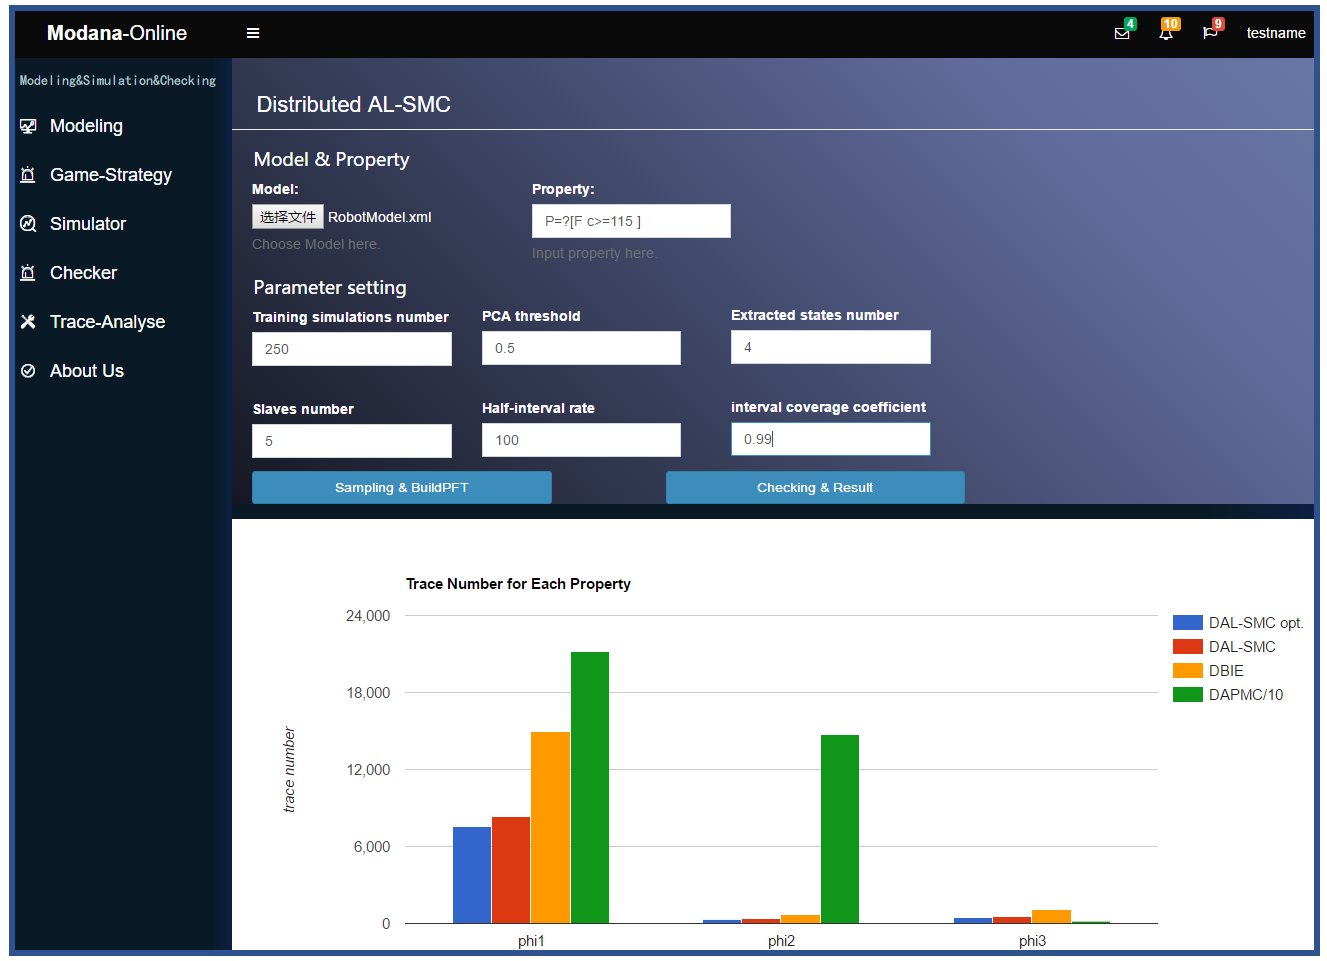
\includegraphics[width=3.2in,height=2.1in]{fig/system.png}}
	%\vspace{0.10in}
	\caption{The user interface of DAL-SMC.}\label{ui_dsmc}
\end{figure}

\subsection{Benchmark experiments}
Uppaal-SMC \cite{Bulychev2012UPPAAL} is a new version of UPPAAL which supports SMC and adopts many SMC algorithms (BHT \cite{jha2009bayesian},SPRT \cite{younes2006statistical}, BIE \cite{zuliani2013bayesian}, APMC \cite{herault2004approximate} etc.). In this paper, we model the benchmark with Uppaal-SMC, and then import the model (.xml) into our platform to verify the properties. Here, we use a simple benchmark to exhibit the distribution of traces in each slave and compare the probability partition between DAL-SMC with parameter optimization (DAL-SMC opt.) and DAL-SMC. Besides, two complex benchmarks are also introduced to compare the efficiency and accuracy among distributed BIE, DAL-SMC, DAL-SMC opt. and distributed APMC (DAPMC) which is a classical quantitative SMC algorithm.

\subsubsection{Train-gate}

A number of trains are approaching a gate on which there is only one track, gate controls the trains to avoid collisions, and restarts them when it is possible to make sure that trains will eventually cross the gate. Figure \ref{train} is the template of the train. Trains delay according to an exponential distribution and synchronize with the gate. The gate keeps track of the trains with an internal queue data structure as shown in Figure \ref{gate}.
\begin{figure*}[htbp]
\centering{
		\subfigure[Train]{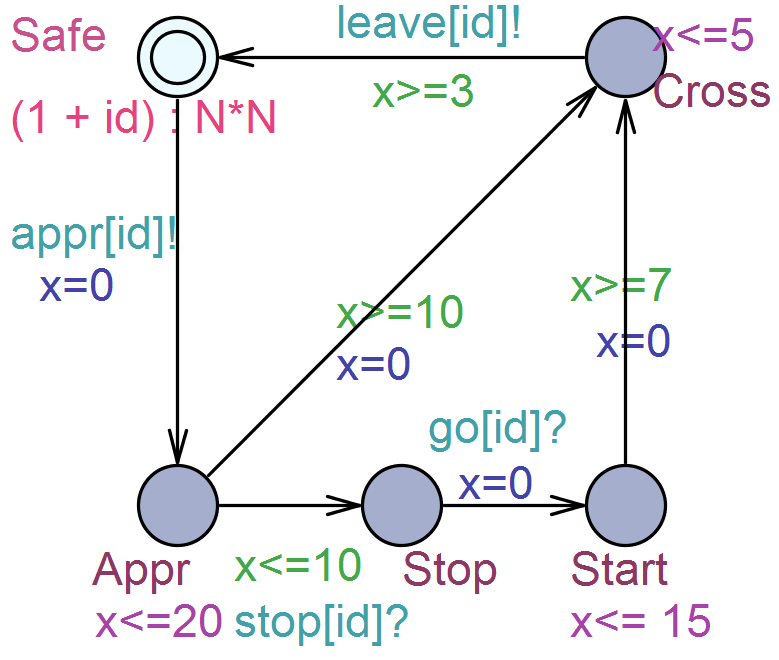
\includegraphics[width=2.0in,height=1.8in]{fig/train.png}
			\label{train}}
		\hfil
		\subfigure[Gate]{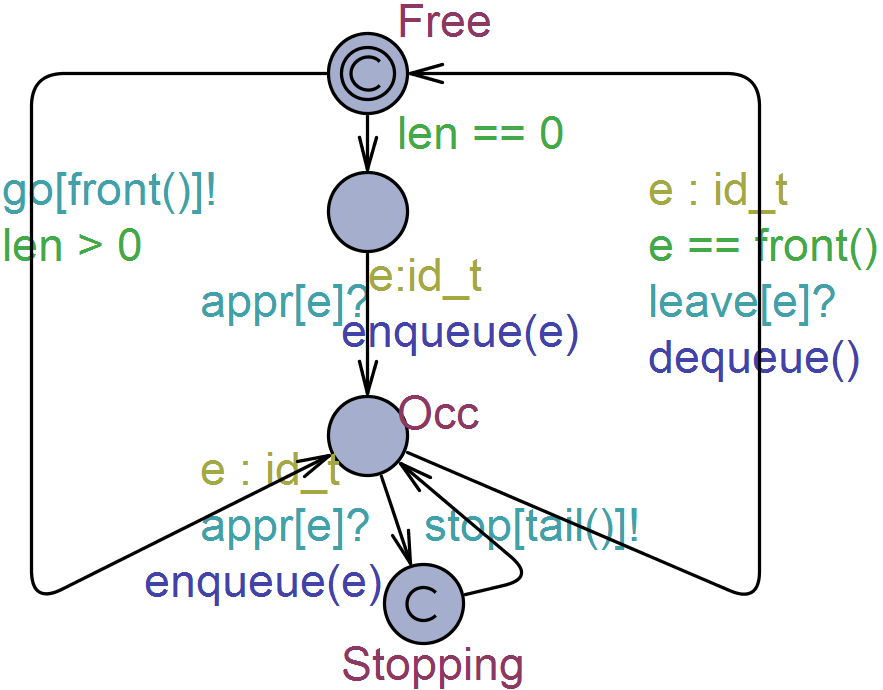
\includegraphics[width=2.5in,height=1.8in]{fig/gate.png}
			\label{gate}}
	\caption{The SHA templates for train-gate.}
	\label{ui_tg}
	}
\end{figure*}
We use Formula \ref{train-proba} to evaluate the probability of Train(0) crossing the gate:
\begin{equation}
P_{=?}(F^{\leq100}~Train(0).Cross)
\label{train-proba}
\end{equation}
\begin{figure}[htbp]
	\centering
	{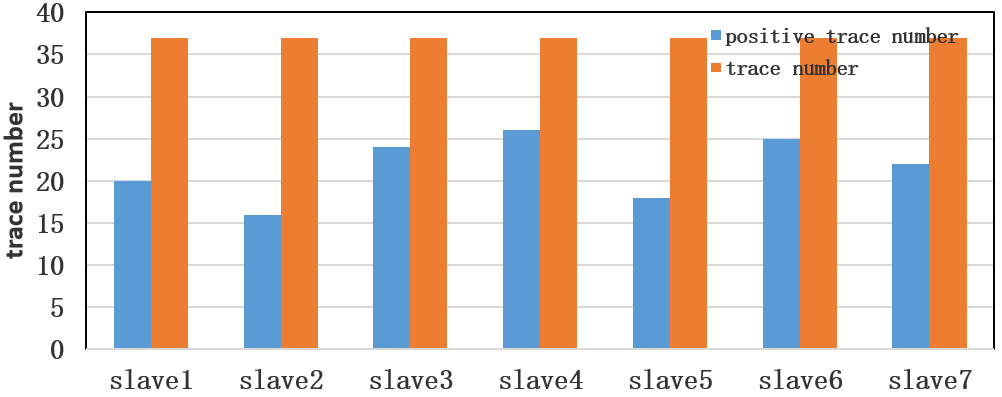
\includegraphics[width=3.2in,height=1.4in]{fig/trace-slave.png}}
	%\vspace{0.10in}
	\caption{Trace number of each slave}
   \label{trace-slave}
\end{figure}
The PBLTL property is used to evaluate the probability interval of Train(0) crossing the gate in 100 time units. The evaluation result is in [0.52707,0.626969] with half-interval size of $\pm0.05$ and interval coverage coefficient of 95\%. We plot the number of traces and satisfying traces of each slave in Figure \ref{trace-slave}. It shows that the slaves generate the same number of traces, however, the number of satisfying traces are not equal. Besides, in order to compare the probability partition between DAL-SMC and DAL-SMC opt, we plot the probability of each sub-space as shown in Figure \ref{BIE-pro}. Figure \ref{pronor} and Figure \ref{proopt} are the probability of each sub-space in DAL-SMC and DAL-SMC opt. respectively. We find that the probability distribution of DAL-SMC opt. is more evenly than that of DAL-SMC, therefore, the parameter optimization is effective. In the next subsections, we will use two complex CPS benchmarks to compare the performance of distributed BIE, DAL-SMC, DAL-SMC opt. and DAPMC.
\begin{figure*}[htbp]
\centering{
		\subfigure[DAL-SMC]{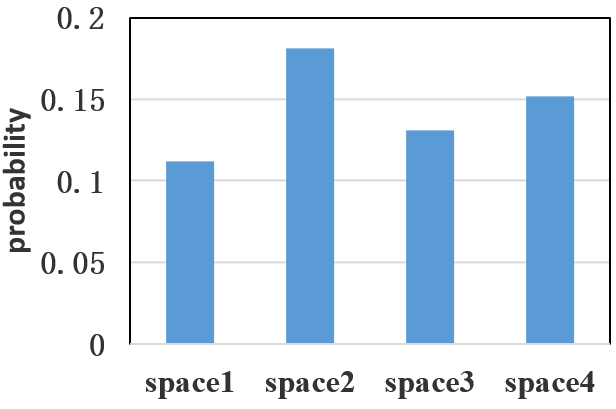
\includegraphics[width=3.0in,height=1.4in]{fig/pro.png}
			\label{pronor}}
		\hfil
		\subfigure[DAL-SMC opt]{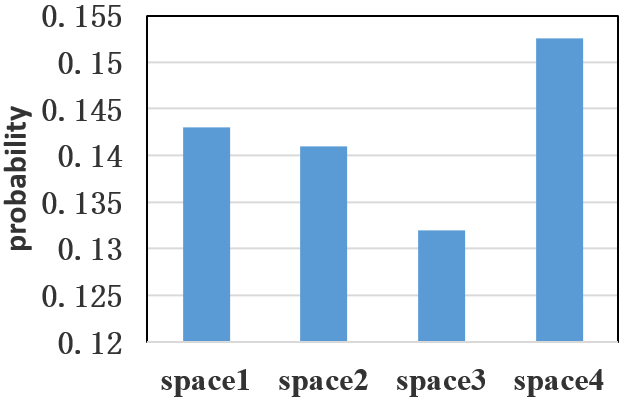
\includegraphics[width=3.0in,height=1.4in]{fig/pro-opt.png}
			\label{proopt}}
	\caption{Probability of each sub-space.}
	\label{BIE-pro}
	}
\end{figure*}

\subsubsection{Energy-aware building}
Energy-aware buildings play an important role in achieving an energy efficient society. The goal is to evaluate and compare the energy consumption of various control strategies with varying environmental settings. There are five SHA models: \emph{room temperature, heater, controller, weather} and \emph{user profile}. Figure \ref{ui_sb} shows the main SHA templates for energy-aware building. In Figure \ref{room}, the room needs to be heated when the temperature is lower than a threshold. The heater moves between locations "Off" and "On" based on the temperature thresholds $on[r]$ and $off[r]$, where r denotes the number of heated room. The central controller decides how to move the heater from one room to another room as shown in Figure \ref{controller}.

\begin{figure*}[htbp]
\centering{
		\subfigure[Room]{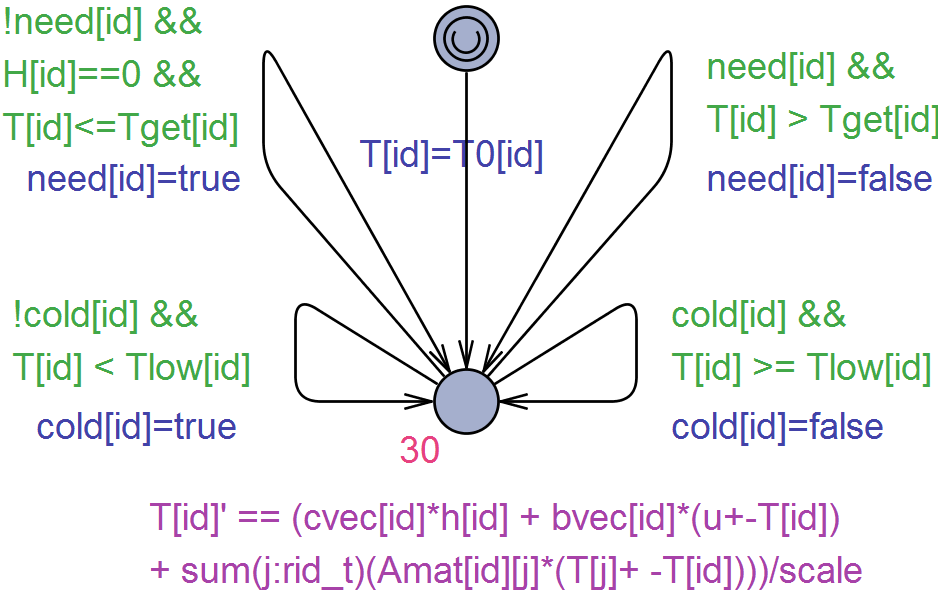
\includegraphics[width=1.8in,height=1.4in]{fig/room.png}
			\label{room}}
		\hfil
		\subfigure[Heater]{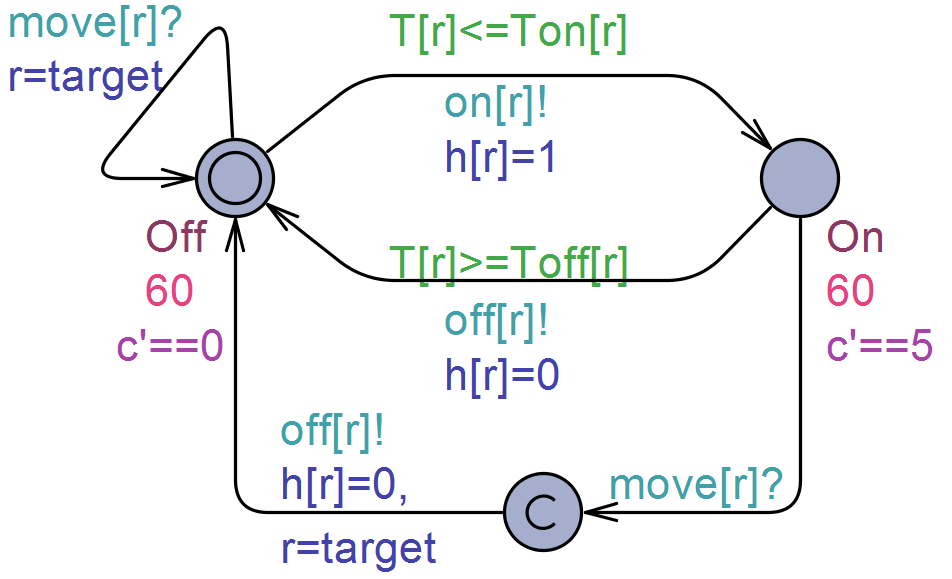
\includegraphics[width=1.8in,height=1.4in]{fig/heater.png}
			\label{heater}}
		\hfil
		\subfigure[Controller]{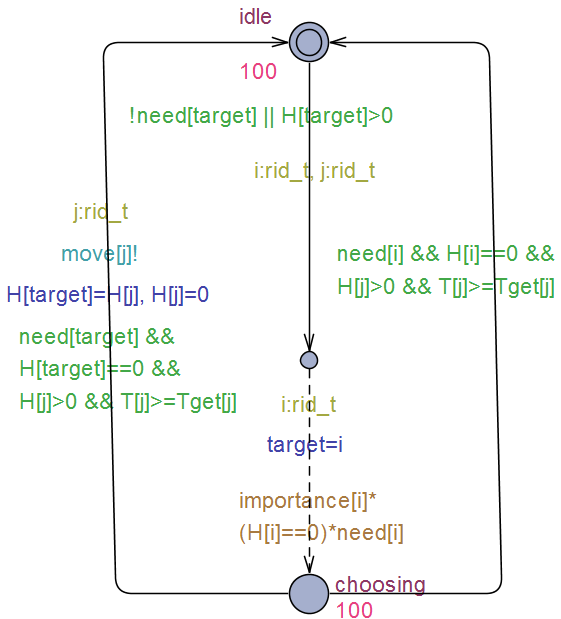
\includegraphics[width=1.5in,height=1.4in]{fig/strategy.png}
			\label{controller}}
	\caption{The main SHA templates for energy-aware building.}
	\label{ui_sb}
	}
\end{figure*}

The experiment has been performed on five slaves on a cluster with Intel Core(TM) i7-4790 (octa-cores at 3.6GHz) interconnected with infiniband. To compare the effciency and accuracy of the algorithms, three properties are verified, which are listed in Table \ref{tb:property}. $\delta$ and $c$ denotes half-interval size and interval coverage coefficient respectively.

\begin{table}[t]
	\renewcommand{\arraystretch}{1.2}
	\caption{Properties of energy-aware building}
	\label{tb:property}
	\centering
	\begin{tabular}{c c l}
		\hline
		~PID~ & $(\delta,c)$ & Property\\
		\hline
		$\phi_1$ & $(0.05,0.99)$ & $P_{=?}(F^{\leq48}~energy \geq 210)$ \\ 
		$\phi_2$ & $(0.01,0.99)$ & $P_{=?}(F^{\leq48}~discomfort \geq 15)$ \\
		$\phi_3$ & $(0.02,0.9)$ & 
		\tabincell{c}{$P_{=?}(F^{\leq48}~ discomfort \leq 15$ \\ $\wedge~energy \geq 170)$} \\
		\hline
	\end{tabular}
\end{table}

We execute each algorithm many times, and compare them in three aspects: the number of traces, time consumption and statistical error. In order to analyse the statistical error of algorithm, we verify the property with high interval coverage coefficient and small half-interval size to obtain the probability ($P_r$). We suppose $P_r$ is the true probability, therefore, the statistical error of each algorithm is $P_r - P_a$, where $P_a$ is the estimation of the true probability. Figure \ref{rs_sb} shows the number of traces, time consumption and statistical error of each algorithm.

\begin{figure*}[htbp]
\centering{
		\subfigure[Trace number of each algorithm]{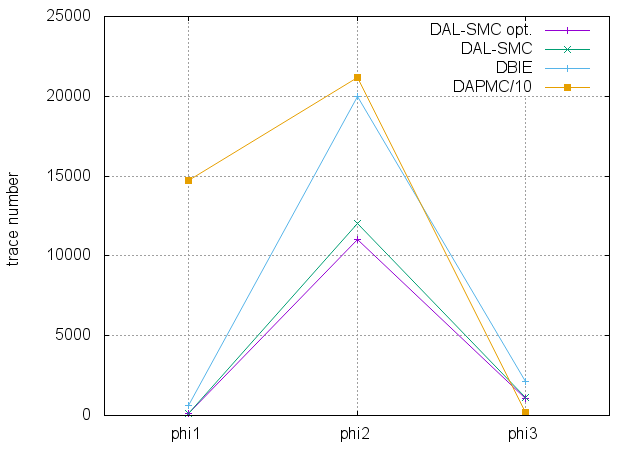
\includegraphics[width=2.0in,height=1.7in]{fig/sb-trace.png}
			\label{trace_sb}}
		\hfil
		\subfigure[Verification time of each algorithm]{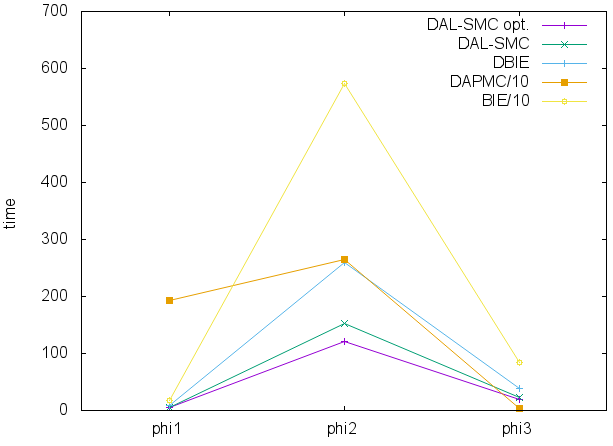
\includegraphics[width=2.0in,height=1.7in]{fig/sb-time.png}
			\label{time_sb}}
		\hfil
		\subfigure[Statistical error of each algorithm]{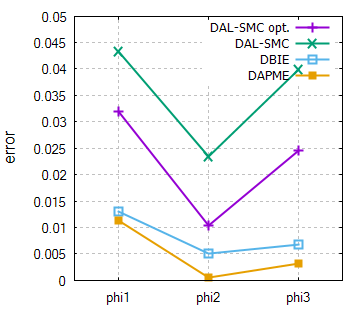
\includegraphics[width=2.0in,height=1.7in]{fig/sb-error.png}
			\label{error_sb}}
	\caption{Algorithms comparison with energy-aware building.}
	\label{rs_sb}
	}
\end{figure*}

Figure \ref{trace_sb} shows the trace number of energy-aware building benchmark generated by each algorithm. We can find that DAPMC algorithm needs 200000 traces to verify property $\phi_2$, however, distributing BIE (DBIE) algorithm only needs 20000 traces. DAL-SMC and DAL-SMC opt. need less traces (about 10000). The time consumption of each algorithm is shown in Figure \ref{time_sb}. The time consumption for verifying property $\phi_2$ with BIE algorithm is 6000 seconds, while it is around 250 seconds consumed by distributed BIE. DAL-SMC and DAL-SMC opt. consume less time. Figure \ref{error_sb} is the statistical error of each algorithm. The statistical error of DAPMC and distributed BIE are about 0.013 for verifying property $\phi1$. The statistical error of DAL-SMC and DAL-SMC opt are about 0.045 and 0.032 respectively. The detailed experiment results are listed in Table \ref{ta-rs}. 

\subsubsection{Robots path planning}

Robots path planning has attracted public attention these years \cite{LWAB10}. The basic goal of a mobile robot is to avoid collision with the moving obstacles, which move irregularly around the environment. As soon as the robot observes the moving obstacle, it will take actions immediately. Different actions consume different energy, so we use some variables to monitor the total energy consumption. Figure \ref{robot-ob} shows the main SHA templates for robot path planning.

\begin{figure*}[htbp]
\centering{
		\subfigure[Robot]{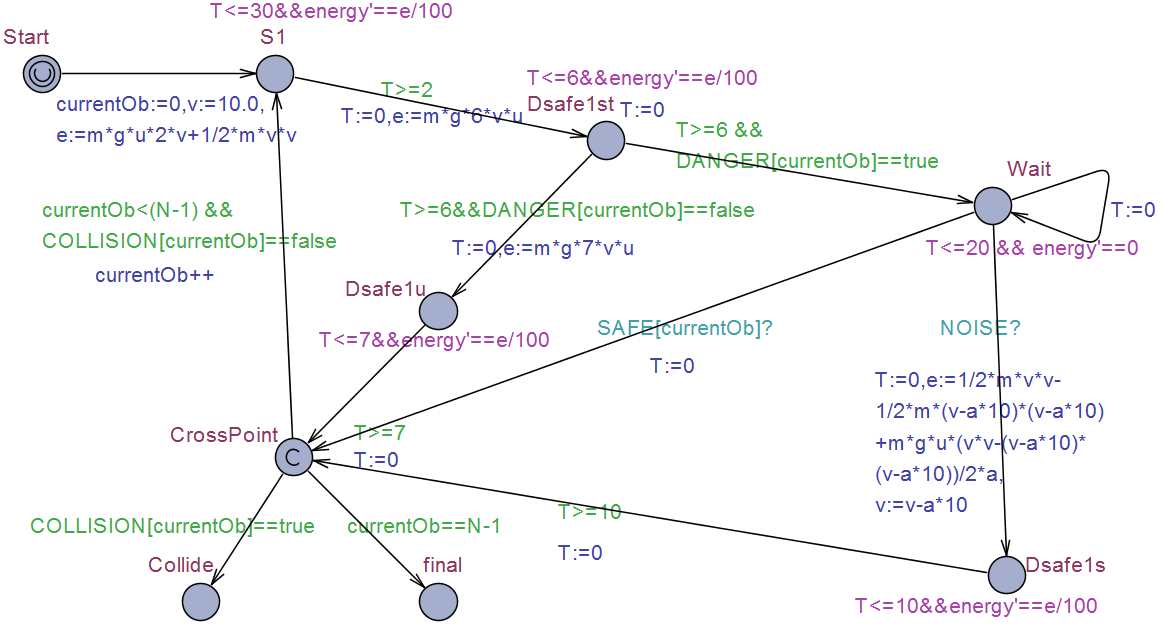
\includegraphics[width=3.0in,height=2.0in]{fig/robot.png}
			\label{robot}}
		\hfil
		\subfigure[Obstacle]{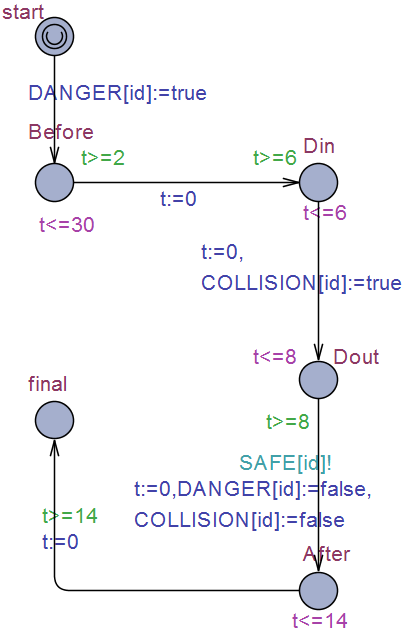
\includegraphics[width=1.5in,height=2.0in]{fig/obstacle.png}
			\label{obstacle}}
	\caption{The main SHA templates for robot path planning.}
	\label{robot-ob}
	}
\end{figure*}


\begin{figure*}[htbp]

\centering{
		\subfigure[Trace number of each algorithm]{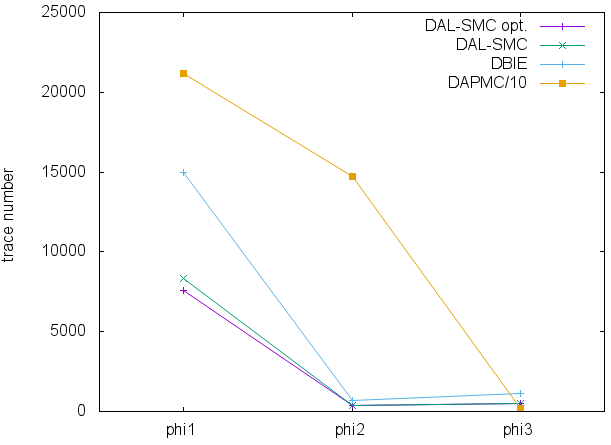
\includegraphics[width=2.0in,height=1.7in]{fig/ro-trace.png}
			\label{trace_ro}}
		\hfil
		\subfigure[Verification time of each algorithm]{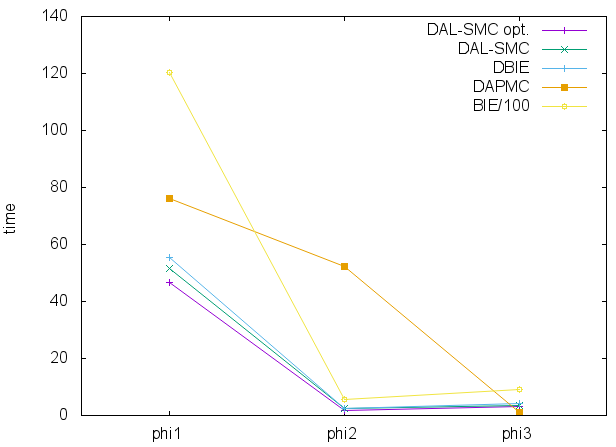
\includegraphics[width=2.0in,height=1.7in]{fig/ro-time.png}
			\label{time_ro}}
		\hfil
		\subfigure[Statistical error of each algorithm]{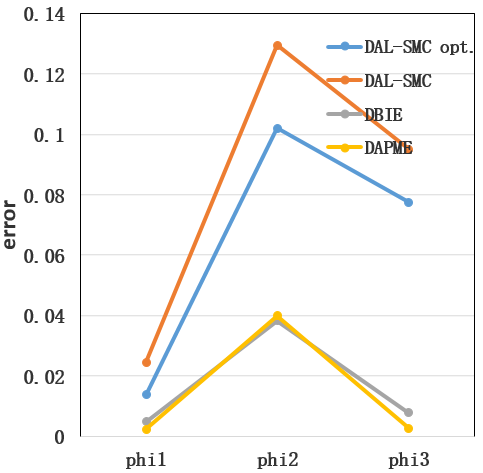
\includegraphics[width=2.0in,height=1.7in]{fig/ro-error.png}
			\label{error_ro}}
	\caption{Algorithms comparison with robots path planning.}
	\label{rs_ro}
	}
\end{figure*}


\begin{table}[t]
	\renewcommand{\arraystretch}{1.2}
	\caption{Properties of robots path planning}
	\label{tb:robot}
	\centering
	\begin{tabular}{c c l}
		\hline
		~PID~ & $(\delta,c)$ & Property\\
		\hline
		$\phi_4$ & $(0.01,0.99)$ & $P_{=?}(F^{\leq100}~robot.collision)$ \\ 
		$\phi_5$ & $(0.05,0.99)$ & $P_{=?}(F^{\leq100}~energy \geq 500)$ \\
		$\phi_6$ & $(0.02,0.9)$ & 
		\tabincell{c}{$P_{=?}(F^{\leq100}~robot.collision$ \\ $\wedge~energy \geq 500)$}\\
		\hline
	\end{tabular}
\end{table}


We also verify three properties $\phi_4$, $\phi_5$, $\phi_6$ for this benchmark as shown in Table \ref{tb:robot}. The experiment results are shown in Figure \ref{rs_ro}. 

In order to analyse the performance of SMC algorithms, the detailed data is listed in Table \ref{ta-rs}. Property $\phi_2$ is verified to illustrate the experimental results, we can conclude that: 

(i)DAPMC generates the most traces for verifying the property, while distributed BIE needs less traces compared with DAPMC. Furthermore, DAL-SMC reduces the number of traces (about 50\%) relative to distributed BIE.  In short, DAL-SMC is the most effective algorithm to generate traces.

(ii)The main time consumption of verification is generating traces (more than 90\%). DAPMC consumes most time, and DAL-SMC consumes less time compared with distributed BIE profitting from less traces. For the benchmark, we use 40 cores to implement distributed algorithms, and we find that the time consumption of BIE algorithm is nearly 25 times as much as distributed BIE which shows it is effective to improve the performance of SMC with distributed techniques. 

(iii)The statistical error of DAPMC and DBIE are similar. The error of DAL-SMC is bigger than that of DAPMC and DBIE due to use multi-BIE. Besides, we find that the error of DAL-SMC opt. is less than that of DAL-SMC. It shows that the parameter optimization method is effective. 

In general, DAL-SMC opt. generates less traces and consumes less time for verification with the help of distributed technology and AL-SMC technique. Meanwhile, the parameter optimization method reduces the statistical error of DAL-SMC to an acceptable range.

\begin{table*}
\caption{Experimental results}
\centering
\begin{tabular}{c c c c c c} 
        \hline  
        Algorithm & Property & Trace Number & Time consumption & Statistical Error\\
        \hline
        \multirow{6}{1.5cm}{DAPMC}  
                & $\phi1(0.05,0.99)$ &  147000&  1934.31&  0.0113\\ 
                & $\phi2(0.01,0.99)$ &  \textbf{211932} &  \textbf{2649.15} &  \textbf{0.0005}\\ 
                & $\phi3(0.02,0.9)$ &  1950&     38.05& 0.0032\\ 
                & $\phi4(0.01,0.99)$ &  211930&  76.282 &  0.0024\\ 
                & $\phi5(0.05,0.99)$ &  147550&  52.206&  0.0399\\ 
                & $\phi6(0.02,0.9)$ &  1850&     1.159& 0.0026\\     
        \hline 
        \multirow{6}{1.5cm}{DBIE}  
                & $\phi1(0.05,0.99)$ &  600&  7.895&  0.0131\\ 
                & $\phi2(0.01,0.99)$ &  \textbf{20000}&  \textbf{259.275} &  \textbf{0.0051} \\ 
                & $\phi3(0.02,0.9)$ &  2100& 38.057& 0.0068\\ 
                & $\phi4(0.01,0.99)$ & 15000&  55.281 &  0.0049\\ 
                & $\phi5(0.05,0.99)$ &  702&  2.483&  0.0382\\ 
                & $\phi6(0.02,0.9)$ &  1120& 4.226& 0.0078\\      
        \hline 
        \multirow{6}{1.5cm}{DAL-SMC}  
                & $\phi1(0.05,0.99)$ &  103&  5.685&  0.0433\\ 
                & $\phi2(0.01,0.99)$ &  \textbf{12000}&  \textbf{151.785} &  \textbf{0.0235} \\ 
                & $\phi3(0.02,0.9)$ &  1137& 22.841& 0.0399\\ 
                & $\phi4(0.01,0.99)$ &  8318&  41.68 &  0.0246\\ 
                & $\phi5(0.05,0.99)$ &  384&  2.32&  0.1295\\ 
                & $\phi6(0.02,0.9)$ &  520& 3.601& \ 0.0751\\      
        \hline 
         \multirow{6}{1.5cm}{DAL-SMC opt.}  
                & $\phi1(0.05,0.99)$ &  95.79&  4.65&  0.0319\\ 
                & $\phi2(0.01,0.99)$ &  \textbf{11040}&  \textbf{121.425} &  \textbf{0.0103}\\ 
                & $\phi3(0.02,0.9)$ &  1091& 18.73& 0.0246\\ 
                & $\phi4(0.01,0.99)$ &  7569&  36.512 &  0.0138\\ 
                & $\phi5(0.05,0.99)$ &  349&  1.81&  0.102\\ 
                & $\phi6(0.02,0.9)$ &  494& 3.171& 0.0575\\     
        \hline 
         \multirow{6}{1.5cm}{BIE}  
                & $\phi1(0.05,0.99)$ &  590&  175.44&  0.0121\\ 
                & $\phi2(0.01,0.99)$ &  \textbf{19586}&  \textbf{5730.67} &  \textbf{0.0047} \\ 
                & $\phi3(0.02,0.9)$ &  2040& 845.73& 0.0063\\ 
                & $\phi4(0.01,0.99)$ & 15400&  1202.467 &  0.0044\\ 
                & $\phi5(0.05,0.99)$ &  762&  55.221&  0.0352\\ 
                & $\phi6(0.02,0.9)$ &  1150& 91.98& 0.0069\\      
        \hline 
\end{tabular} 
\label{ta-rs}
\end{table*}



\section{Related Works}
Statistical Model Checking technique was first proposed by R.Grosu \cite{grosu2005monte}. Some variations \cite{legay2010statistical} \cite{Younes2004Planning} \cite{younes2006statistical}\cite{jha2009bayesian} \cite{zuliani2013bayesian} \cite{herault2004} based on the basic SMC have been proposed in the past few years. Some related work are summarized as follows:

\textbf{Basic SMC.}
SMC refers to a series of simulation-based techniques that can be used to answer two questions: (1)Qualitative: Is the probability of model \emph{s} satisfying property $\phi$ greater than or equal to a certain threshold? and (2)Quantitative: What is the probability of model \emph{s} satisfying property $\phi$? For qualitative SMC, Kim.G.larsn et al. \cite{kim2012statistical} have given an empirical evaluation. BHT and SPRT are more effective than SSP. BHT generates more traces when checking the property whose estimation probability is close to its real probability, so SPRT is faster than BHT for this situation. For other situation, BHT is obviously more efficient than SPRT. For quantitative SMC, Zuliani et al. \cite{zuliani2013bayesian} have compared the number of traces analyzed by APMC and BIE, and they have concluded that BIE excels remarkably in performance. Our approach focuses on the performance of BIE algorithm.

\textbf{SMC with abstraction and learning.}
BIE algorithm needs more traces when checking the property whose probability is close to 0.5, while the number of traces is drastically reduced when the probability approaches to 0 or 1 \cite{zuliani2013bayesian}. In our recent work \cite{jiangkaiqiang2016}, we have partitioned the original probability space $\Omega$ into many sub-spaces $\Omega_1$,... ,$\Omega_m$, and evaluated the probability of each sub-space in parallel. Therefore, the trace number for evaluating the original probability will be decreased and depends on the maximum number of traces for evaluating sub-spaces theoretically. We find that the number of traces is effectively reduced while ensuring the accuracy of the probability within an acceptable error bound.

\textbf{Distributed SMC.}
As observed in \cite{younes2005ymer}, SMC algorithms can be distributed with master/slave architecture where multiple slave processes are used to generate traces. When working with an estimation algorithm, the number of traces for verifying the property is known in advance and can be equally distributed between the slaves. When working with the sequential algorithms, the situation gets more complicated, so we need to avoid introducing bias when collecting the traces generated by the slave processes. To solve this problem, H. L. S. Younes proposed a method in \cite{Younes2004Planning} where the bias is avoided by committing ,$\alpha$ $priori$, to the order in which observations will be taken into account. Peter Bulychev et al. generalized the above method with batches and buffer \cite{Bulychev2012Checking}. Batches aggregate the outcomes for reducing communication and the buffer is used to improve concurrency since the nodes are more loosely synchronized. They also implemented the distributed Hypothesis testing algorithm without introducing bias. The algorithm effectively reduce the time consumption for generating a single trace. Our work is different from the existing work, we use abstraction and learning technique (AL-SMC) to reduce the number of simulation traces, and adopt distributed technology with AL-SMC to reduce both the number of traces and time consumption for generating a single traces.   
\section{Conclusion and Future Work}
\label{sec:conclusion&ack}
This paper has presented our novel approach to check the FMI co-simulation , which facilitates the formal analysis of CPSs. This involves model checking the reachability, livelock and deadlock of three various master algorithms. Besides, the correctness and  relevant system properties of the architecture are also analysed. To achieve the goal, we encode the FMU and master algorithms with timed automata. Then the properties of the co-simulation are verified with UPPAAL. We evaluate this approach using the example water tank. The results show that our approach is feasible and useful.

An interesting direction of future work is that we attempt to analyse and compare the performance of various master algorithms in the future. Besides, more complex case studies will be conducted to check the scalability of proposed approach. The tool support for our approach should be improved further.
\section*{Acknowledgement}
This work was supported by NSFC (Grant No.61472140, 61202104) and NSF of Shanghai (Grant No. 14ZR1412500).






% BibTeX users please use one of
%\bibliographystyle{spbasic}      % basic style, author-year citations
%\bibliographystyle{spmpsci}      % mathematics and physical sciences
%\bibliographystyle{spphys}       % APS-like style for physics
%\bibliography{}   % name your BibTeX data base


% Bibliography
\bibliographystyle{spmpsci}
\bibliography{sample-bibliography}



% Non-BibTeX users please use
%\begin{thebibliography}{}
%
% and use \bibitem to create references. Consult the Instructions
% for authors for reference list style.
%

% Format for books
%\bibitem{RefB}
%Author, Book title, page numbers. Publisher, place (year)
% etc
%\end{thebibliography}

\end{document}
% end of file template.tex

